\documentclass{article}

\usepackage[english]{babel}

\usepackage[a4paper,top=2cm,bottom=2cm,left=3cm,right=3cm,marginparwidth=1.75cm]{geometry}

% Useful packages
\usepackage{amsmath}
\usepackage{graphicx}
\usepackage[colorlinks=true, allcolors=blue]{hyperref}

\title{Your Paper}
\author{You}

\begin{document}
\maketitle

\begin{abstract}
Your abstract.
\end{abstract}

\section{Introduction}

An image is shown at Figure \ref{fig:Icebear}, cf. \cite{icebear}.

\begin{figure}[h!]
\centering
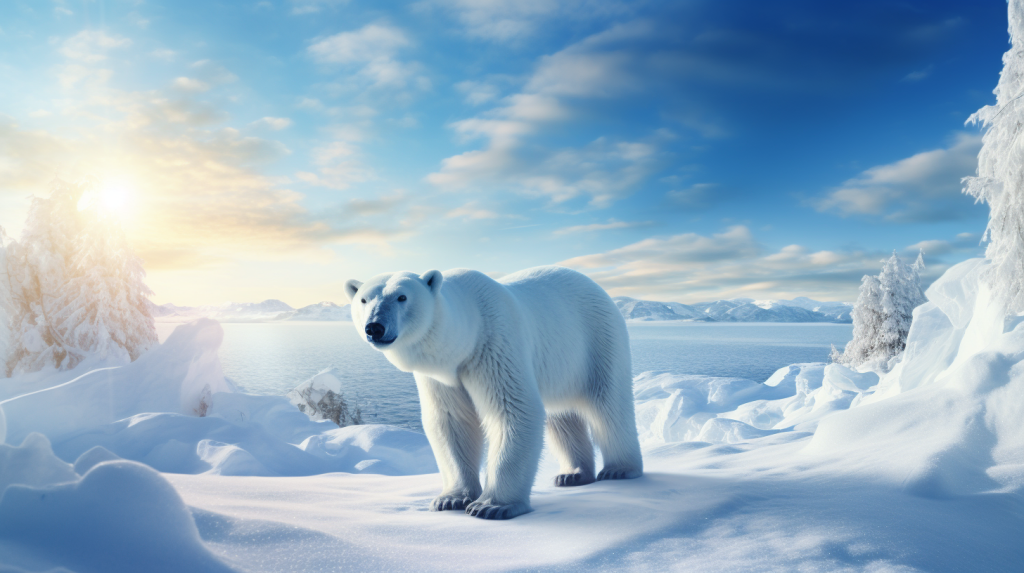
\includegraphics[width=\linewidth]{images/icebear}
\caption{\label{fig:Icebear} Icebear.}
\end{figure}

\bibliographystyle{alpha}
\bibliography{bib}

\end{document}
